% Figure 2. What electrical engineers earn. Labels: LABELS.md, Figure 2.
% The bar is drawn to scale: left end $76,550, right end $120,630, marker $87,853.
\def\eeprepfigure{1}
\providecommand{\eepstyledir}{../style}% repo: ../style
\input{\eepstyledir/circuitikz-preamble.tex}
% Colours, fonts, and text styles for the Get hired figures.
% Input after style/circuitikz-preamble.tex (in the repo: ../../style/circuitikz-preamble.tex).
% Define \eepdark before this file for the dark build. Same names as the resume figures,
% plus the rest of the navy palette. Crimson (eepaccent) marks one thing per figure.
\setmainfont{Newsreader}[
  BoldFont={Newsreader Bold},
  ItalicFont={Newsreader Italic},
  BoldItalicFont={Newsreader Bold Italic},
]
\usetikzlibrary{arrows.meta,calc,decorations.pathreplacing}
\ifdefined\eepdark
  \definecolor{eepink}{HTML}{ECEEF2}
  \definecolor{eeptext}{HTML}{D0D4DB}
  \definecolor{eepinktwo}{HTML}{A6AFBF}
  \definecolor{eepmute}{HTML}{8F95A0}
  \definecolor{eepsilver}{HTML}{76808F}
  \definecolor{eeprule}{HTML}{3B4352}
  \definecolor{eepwash}{HTML}{17243A}
  \definecolor{eepsunken}{HTML}{101828}
  \definecolor{eepfill}{HTML}{131C2E}
  \definecolor{eeppaper}{HTML}{0D1524}
  \definecolor{eepaccent}{HTML}{E06A5F}
  \definecolor{eepaccentsoft}{HTML}{2A1A24}
\else
  \definecolor{eepink}{HTML}{16233A}
  \definecolor{eeptext}{HTML}{232A39}
  \definecolor{eepinktwo}{HTML}{424D63}
  \definecolor{eepmute}{HTML}{5E636C}
  \definecolor{eepsilver}{HTML}{838C9A}
  \definecolor{eeprule}{HTML}{C4C8CF}
  \definecolor{eepwash}{HTML}{E7ECF3}
  \definecolor{eepsunken}{HTML}{F3F4F6}
  \definecolor{eepfill}{HTML}{FFFFFF}
  \definecolor{eeppaper}{HTML}{FBFBFC}
  \definecolor{eepaccent}{HTML}{A3201D}
  \definecolor{eepaccentsoft}{HTML}{F8ECEA}
\fi
% Draw in y-down points so coordinates read like a mockup: [x=1pt, y=-1pt].
\tikzset{
  eeptitle/.style={anchor=base west, inner sep=0pt, text=eepink, font=\rmfamily\bfseries\fontsize{26}{31}\selectfont},
  eephead/.style={inner sep=0pt, text=eepink, font=\sffamily\bfseries\fontsize{14.5}{18}\selectfont},
  eepbody/.style={inner sep=0pt, text=eepinktwo, font=\sffamily\fontsize{13}{17}\selectfont},
  eepnote/.style={inner sep=0pt, text=eepmute, font=\sffamily\fontsize{12.5}{16}\selectfont},
  eepsrc/.style={anchor=north west, inner sep=0pt, align=left, text=eepmute, font=\sffamily\fontsize{11}{14.5}\selectfont},
  eepbox/.style={draw=eepink, fill=eepfill, rounded corners=4pt},
  eepfocus/.style={draw=eepaccent, fill=eepfill, rounded corners=4pt, line width=1.8pt},
  eeparrow/.style={-{Stealth[length=8pt,width=6pt]}},
  eepdash/.style={dash pattern=on 4pt off 4pt},
  eeplead/.style={draw=eepsilver, line width=0.9pt},
}
% A dot on a trace, like a schematic junction.
\newcommand{\eepdot}[2][eepink]{\fill[#1] #2 circle (3.6pt);}
% Short labels never hyphenate.
\hyphenpenalty=10000 \exhyphenpenalty=10000
% One space after a full stop, as on the site.
\frenchspacing

\begin{document}
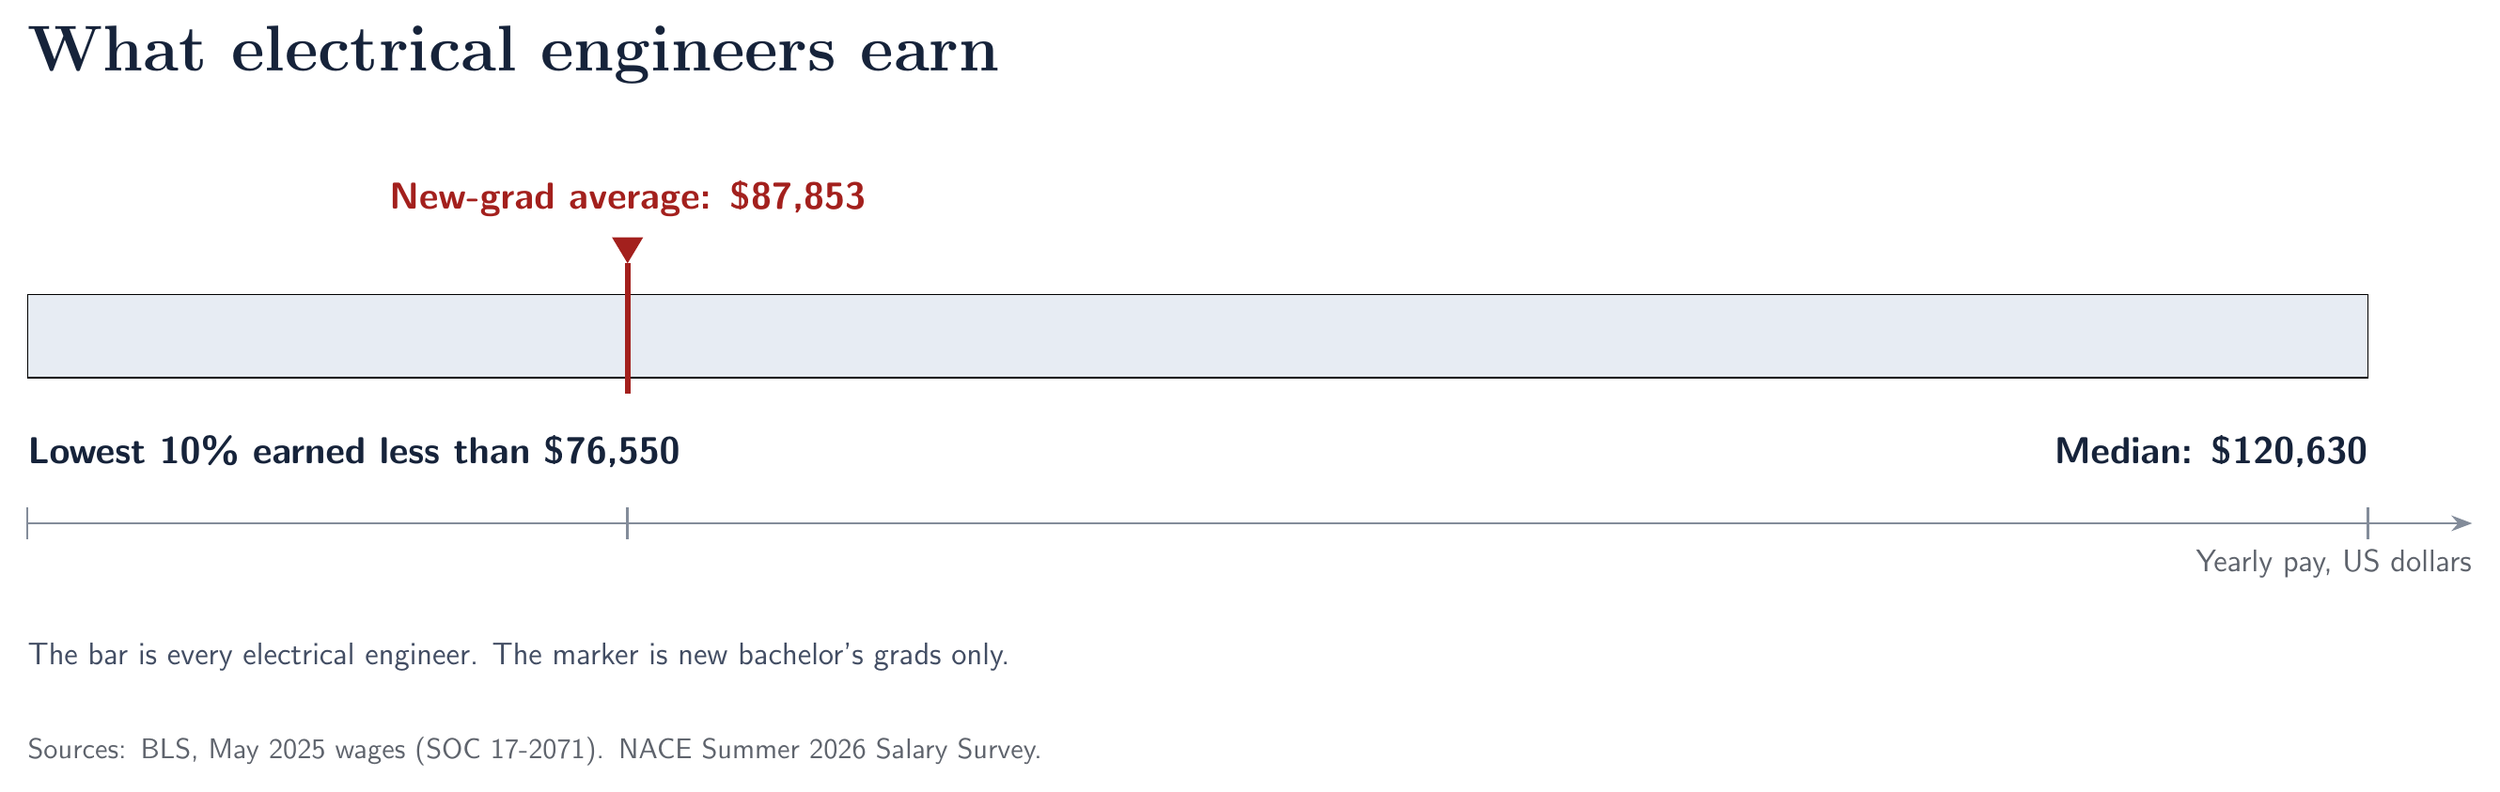
\begin{tikzpicture}[x=1pt,y=-1pt]
  \def\barw{900}
  \pgfmathsetmacro\mk{(87.853-76.550)/(120.630-76.550)*\barw}% thousands, to stay inside TeX dimensions
  \node[eeptitle] at (0,30) {What electrical engineers earn};
  % The bar: every electrical engineer, lowest 10% line to median.
  \draw[fill=eepwash] (0,116) rectangle (\barw,148);
  % End labels.
  \node[eephead, anchor=north west] at (0,170) {Lowest 10\% earned less than \$76,550};
  \node[eephead, anchor=north east] at (\barw,170) {Median: \$120,630};
  % Axis, with a tick at each value on the figure.
  \draw[eepsilver, line width=1pt, eeparrow] (0,204) -- (\barw+40,204);
  \foreach \x in {0,\mk,\barw} \draw[eepsilver, line width=1pt] (\x,198) -- (\x,210);
  \node[eepnote, anchor=north east] at (\barw+40,214) {Yearly pay, US dollars};
  % The marker: new bachelor's grads only.
  \draw[eepaccent, line width=2.2pt] (\mk,104) -- (\mk,154);
  \fill[eepaccent] (\mk-6,94) -- (\mk+6,94) -- (\mk,104) -- cycle;
  \node[eephead, text=eepaccent, anchor=south] at (\mk,86) {New-grad average: \$87,853};
  \node[eepbody, anchor=north west] at (0,250) {The bar is every electrical engineer. The marker is new bachelor's grads only.};
  \node[eepsrc, text width=940pt] at (0,286) {Sources: BLS, May 2025 wages (SOC 17-2071). NACE Summer 2026 Salary Survey.};
\end{tikzpicture}
\end{document}
